\documentclass{article}
% Configuration for the memoir class.
\renewcommand{\cleardoublepage}{}
% \renewcommand*{\partpageend}{}
\renewcommand{\afterpartskip}{}
\maxsecnumdepth{subsubsection} % number subsections
\maxtocdepth{subsubsection}

\addtolength{\parindent}{-5mm}
% Packages not included:
% For multiline comments, use caption package. But this conflicts with hyperref while making html files.
% subfigure conflicts with use with memoir style-sheet.

% Use something like:
% % Use something like:
% % Use something like:
% \input{../../macros}

% groupings of objects.
\newcommand{\set}[1]{\left\{ #1 \right\}}
\newcommand{\seq}[1]{\left(#1\right)}
\newcommand{\ang}[1]{\langle#1\rangle}
\newcommand{\tuple}[1]{\left(#1\right)}

% numerical shortcuts.
\newcommand{\abs}[1]{\left| #1\right|}
\newcommand{\floor}[1]{\left\lfloor #1 \right\rfloor}
\newcommand{\ceil}[1]{\left\lceil #1 \right\rceil}

% linear algebra shortcuts.
\newcommand{\change}{\Delta}
\newcommand{\norm}[1]{\left\| #1\right\|}
\newcommand{\dprod}[1]{\langle#1\rangle}
\newcommand{\linspan}[1]{\langle#1\rangle}
\newcommand{\conj}[1]{\overline{#1}}
\newcommand{\gradient}{\nabla}
\newcommand{\der}{\frac{d}{dx}}
\newcommand{\lap}{\Delta}
\newcommand{\kron}{\otimes}
\newcommand{\nperp}{\nvdash}

\newcommand{\mat}[1]{\left( \begin{smallmatrix}#1 \end{smallmatrix} \right)}

% derivatives and limits
\newcommand{\partder}[2]{\frac{\partial #1}{\partial #2}}
\newcommand{\partdern}[3]{\frac{\partial^{#3} #1}{\partial #2^{#3}}}

% Arrows
\newcommand{\diverge}{\nearrow}
\newcommand{\notto}{\nrightarrow}
\newcommand{\up}{\uparrow}
\newcommand{\down}{\downarrow}
% gets and gives are defined!

% ordering operators
\newcommand{\oleq}{\preceq}
\newcommand{\ogeq}{\succeq}

% programming and logic operators
\newcommand{\dfn}{:=}
\newcommand{\assign}{:=}
\newcommand{\co}{\ co\ }
\newcommand{\en}{\ en\ }


% logic operators
\newcommand{\xor}{\oplus}
\newcommand{\Land}{\bigwedge}
\newcommand{\Lor}{\bigvee}
\newcommand{\finish}{$\Box$}
\newcommand{\contra}{\Rightarrow \Leftarrow}
\newcommand{\iseq}{\stackrel{_?}{=}}


% Set theory
\newcommand{\symdiff}{\Delta}
\newcommand{\union}{\cup}
\newcommand{\inters}{\cap}
\newcommand{\Union}{\bigcup}
\newcommand{\Inters}{\bigcap}
\newcommand{\nullSet}{\phi}

% graph theory
\newcommand{\nbd}{\Gamma}

% Script alphabets
% For reals, use \Re

% greek letters
\newcommand{\eps}{\epsilon}
\newcommand{\del}{\delta}
\newcommand{\ga}{\alpha}
\newcommand{\gb}{\beta}
\newcommand{\gd}{\del}
\newcommand{\gf}{\phi}
\newcommand{\gF}{\Phi}
\newcommand{\gl}{\lambda}
\newcommand{\gm}{\mu}
\newcommand{\gn}{\nu}
\newcommand{\gr}{\rho}
\newcommand{\gs}{\sigma}
\newcommand{\gt}{\theta}
\newcommand{\gx}{\xi}

\newcommand{\sw}{\sigma}
\newcommand{\SW}{\Sigma}
\newcommand{\ew}{\lambda}
\newcommand{\EW}{\Lambda}

\newcommand{\Del}{\Delta}
\newcommand{\gD}{\Delta}
\newcommand{\gG}{\Gamma}
\newcommand{\gO}{\Omega}
\newcommand{\gL}{\Lambda}
\newcommand{\gS}{\Sigma}

% Formatting shortcuts
\newcommand{\red}[1]{\textcolor{red}{#1}}
\newcommand{\blue}[1]{\textcolor{blue}{#1}}
\newcommand{\htext}[2]{\texorpdfstring{#1}{#2}}

% Statistics
\newcommand{\distr}{\sim}
\newcommand{\stddev}{\sigma}
\newcommand{\covmatrix}{\Sigma}
\newcommand{\mean}{\mu}
\newcommand{\param}{\gt}
\newcommand{\ftr}{\phi}

% General utility
\newcommand{\todo}[1]{\footnote{TODO: #1}}
\newcommand{\exclaim}[1]{{\textbf{\textit{#1}}}}
\newcommand{\tbc}{[\textbf{Incomplete}]}
\newcommand{\chk}{[\textbf{Check}]}
\newcommand{\oprob}{[\textbf{OP}]:}
\newcommand{\core}[1]{\textbf{Core Idea:}}
\newcommand{\why}{[\textbf{Find proof}]}
\newcommand{\opt}[1]{\textit{#1}}


\DeclareMathOperator*{\argmin}{arg\,min}
\DeclareMathOperator{\rank}{rank}
\newcommand{\redcol}[1]{\textcolor{red}{#1}}
\newcommand{\bluecol}[1]{\textcolor{blue}{#1}}
\newcommand{\greencol}[1]{\textcolor{green}{#1}}


\renewcommand{\~}{\htext{$\sim$}{~}}


% groupings of objects.
\newcommand{\set}[1]{\left\{ #1 \right\}}
\newcommand{\seq}[1]{\left(#1\right)}
\newcommand{\ang}[1]{\langle#1\rangle}
\newcommand{\tuple}[1]{\left(#1\right)}

% numerical shortcuts.
\newcommand{\abs}[1]{\left| #1\right|}
\newcommand{\floor}[1]{\left\lfloor #1 \right\rfloor}
\newcommand{\ceil}[1]{\left\lceil #1 \right\rceil}

% linear algebra shortcuts.
\newcommand{\change}{\Delta}
\newcommand{\norm}[1]{\left\| #1\right\|}
\newcommand{\dprod}[1]{\langle#1\rangle}
\newcommand{\linspan}[1]{\langle#1\rangle}
\newcommand{\conj}[1]{\overline{#1}}
\newcommand{\gradient}{\nabla}
\newcommand{\der}{\frac{d}{dx}}
\newcommand{\lap}{\Delta}
\newcommand{\kron}{\otimes}
\newcommand{\nperp}{\nvdash}

\newcommand{\mat}[1]{\left( \begin{smallmatrix}#1 \end{smallmatrix} \right)}

% derivatives and limits
\newcommand{\partder}[2]{\frac{\partial #1}{\partial #2}}
\newcommand{\partdern}[3]{\frac{\partial^{#3} #1}{\partial #2^{#3}}}

% Arrows
\newcommand{\diverge}{\nearrow}
\newcommand{\notto}{\nrightarrow}
\newcommand{\up}{\uparrow}
\newcommand{\down}{\downarrow}
% gets and gives are defined!

% ordering operators
\newcommand{\oleq}{\preceq}
\newcommand{\ogeq}{\succeq}

% programming and logic operators
\newcommand{\dfn}{:=}
\newcommand{\assign}{:=}
\newcommand{\co}{\ co\ }
\newcommand{\en}{\ en\ }


% logic operators
\newcommand{\xor}{\oplus}
\newcommand{\Land}{\bigwedge}
\newcommand{\Lor}{\bigvee}
\newcommand{\finish}{$\Box$}
\newcommand{\contra}{\Rightarrow \Leftarrow}
\newcommand{\iseq}{\stackrel{_?}{=}}


% Set theory
\newcommand{\symdiff}{\Delta}
\newcommand{\union}{\cup}
\newcommand{\inters}{\cap}
\newcommand{\Union}{\bigcup}
\newcommand{\Inters}{\bigcap}
\newcommand{\nullSet}{\phi}

% graph theory
\newcommand{\nbd}{\Gamma}

% Script alphabets
% For reals, use \Re

% greek letters
\newcommand{\eps}{\epsilon}
\newcommand{\del}{\delta}
\newcommand{\ga}{\alpha}
\newcommand{\gb}{\beta}
\newcommand{\gd}{\del}
\newcommand{\gf}{\phi}
\newcommand{\gF}{\Phi}
\newcommand{\gl}{\lambda}
\newcommand{\gm}{\mu}
\newcommand{\gn}{\nu}
\newcommand{\gr}{\rho}
\newcommand{\gs}{\sigma}
\newcommand{\gt}{\theta}
\newcommand{\gx}{\xi}

\newcommand{\sw}{\sigma}
\newcommand{\SW}{\Sigma}
\newcommand{\ew}{\lambda}
\newcommand{\EW}{\Lambda}

\newcommand{\Del}{\Delta}
\newcommand{\gD}{\Delta}
\newcommand{\gG}{\Gamma}
\newcommand{\gO}{\Omega}
\newcommand{\gL}{\Lambda}
\newcommand{\gS}{\Sigma}

% Formatting shortcuts
\newcommand{\red}[1]{\textcolor{red}{#1}}
\newcommand{\blue}[1]{\textcolor{blue}{#1}}
\newcommand{\htext}[2]{\texorpdfstring{#1}{#2}}

% Statistics
\newcommand{\distr}{\sim}
\newcommand{\stddev}{\sigma}
\newcommand{\covmatrix}{\Sigma}
\newcommand{\mean}{\mu}
\newcommand{\param}{\gt}
\newcommand{\ftr}{\phi}

% General utility
\newcommand{\todo}[1]{\footnote{TODO: #1}}
\newcommand{\exclaim}[1]{{\textbf{\textit{#1}}}}
\newcommand{\tbc}{[\textbf{Incomplete}]}
\newcommand{\chk}{[\textbf{Check}]}
\newcommand{\oprob}{[\textbf{OP}]:}
\newcommand{\core}[1]{\textbf{Core Idea:}}
\newcommand{\why}{[\textbf{Find proof}]}
\newcommand{\opt}[1]{\textit{#1}}


\DeclareMathOperator*{\argmin}{arg\,min}
\DeclareMathOperator{\rank}{rank}
\newcommand{\redcol}[1]{\textcolor{red}{#1}}
\newcommand{\bluecol}[1]{\textcolor{blue}{#1}}
\newcommand{\greencol}[1]{\textcolor{green}{#1}}


\renewcommand{\~}{\htext{$\sim$}{~}}


% groupings of objects.
\newcommand{\set}[1]{\left\{ #1 \right\}}
\newcommand{\seq}[1]{\left(#1\right)}
\newcommand{\ang}[1]{\langle#1\rangle}
\newcommand{\tuple}[1]{\left(#1\right)}

% numerical shortcuts.
\newcommand{\abs}[1]{\left| #1\right|}
\newcommand{\floor}[1]{\left\lfloor #1 \right\rfloor}
\newcommand{\ceil}[1]{\left\lceil #1 \right\rceil}

% linear algebra shortcuts.
\newcommand{\change}{\Delta}
\newcommand{\norm}[1]{\left\| #1\right\|}
\newcommand{\dprod}[1]{\langle#1\rangle}
\newcommand{\linspan}[1]{\langle#1\rangle}
\newcommand{\conj}[1]{\overline{#1}}
\newcommand{\gradient}{\nabla}
\newcommand{\der}{\frac{d}{dx}}
\newcommand{\lap}{\Delta}
\newcommand{\kron}{\otimes}
\newcommand{\nperp}{\nvdash}

\newcommand{\mat}[1]{\left( \begin{smallmatrix}#1 \end{smallmatrix} \right)}

% derivatives and limits
\newcommand{\partder}[2]{\frac{\partial #1}{\partial #2}}
\newcommand{\partdern}[3]{\frac{\partial^{#3} #1}{\partial #2^{#3}}}

% Arrows
\newcommand{\diverge}{\nearrow}
\newcommand{\notto}{\nrightarrow}
\newcommand{\up}{\uparrow}
\newcommand{\down}{\downarrow}
% gets and gives are defined!

% ordering operators
\newcommand{\oleq}{\preceq}
\newcommand{\ogeq}{\succeq}

% programming and logic operators
\newcommand{\dfn}{:=}
\newcommand{\assign}{:=}
\newcommand{\co}{\ co\ }
\newcommand{\en}{\ en\ }


% logic operators
\newcommand{\xor}{\oplus}
\newcommand{\Land}{\bigwedge}
\newcommand{\Lor}{\bigvee}
\newcommand{\finish}{$\Box$}
\newcommand{\contra}{\Rightarrow \Leftarrow}
\newcommand{\iseq}{\stackrel{_?}{=}}


% Set theory
\newcommand{\symdiff}{\Delta}
\newcommand{\union}{\cup}
\newcommand{\inters}{\cap}
\newcommand{\Union}{\bigcup}
\newcommand{\Inters}{\bigcap}
\newcommand{\nullSet}{\phi}

% graph theory
\newcommand{\nbd}{\Gamma}

% Script alphabets
% For reals, use \Re

% greek letters
\newcommand{\eps}{\epsilon}
\newcommand{\del}{\delta}
\newcommand{\ga}{\alpha}
\newcommand{\gb}{\beta}
\newcommand{\gd}{\del}
\newcommand{\gf}{\phi}
\newcommand{\gF}{\Phi}
\newcommand{\gl}{\lambda}
\newcommand{\gm}{\mu}
\newcommand{\gn}{\nu}
\newcommand{\gr}{\rho}
\newcommand{\gs}{\sigma}
\newcommand{\gt}{\theta}
\newcommand{\gx}{\xi}

\newcommand{\sw}{\sigma}
\newcommand{\SW}{\Sigma}
\newcommand{\ew}{\lambda}
\newcommand{\EW}{\Lambda}

\newcommand{\Del}{\Delta}
\newcommand{\gD}{\Delta}
\newcommand{\gG}{\Gamma}
\newcommand{\gO}{\Omega}
\newcommand{\gL}{\Lambda}
\newcommand{\gS}{\Sigma}

% Formatting shortcuts
\newcommand{\red}[1]{\textcolor{red}{#1}}
\newcommand{\blue}[1]{\textcolor{blue}{#1}}
\newcommand{\htext}[2]{\texorpdfstring{#1}{#2}}

% Statistics
\newcommand{\distr}{\sim}
\newcommand{\stddev}{\sigma}
\newcommand{\covmatrix}{\Sigma}
\newcommand{\mean}{\mu}
\newcommand{\param}{\gt}
\newcommand{\ftr}{\phi}

% General utility
\newcommand{\todo}[1]{\footnote{TODO: #1}}
\newcommand{\exclaim}[1]{{\textbf{\textit{#1}}}}
\newcommand{\tbc}{[\textbf{Incomplete}]}
\newcommand{\chk}{[\textbf{Check}]}
\newcommand{\oprob}{[\textbf{OP}]:}
\newcommand{\core}[1]{\textbf{Core Idea:}}
\newcommand{\why}{[\textbf{Find proof}]}
\newcommand{\opt}[1]{\textit{#1}}


\DeclareMathOperator*{\argmin}{arg\,min}
\DeclareMathOperator{\rank}{rank}
\newcommand{\redcol}[1]{\textcolor{red}{#1}}
\newcommand{\bluecol}[1]{\textcolor{blue}{#1}}
\newcommand{\greencol}[1]{\textcolor{green}{#1}}


\renewcommand{\~}{\htext{$\sim$}{~}}



%opening
\title{Data mining: Homework 2}
\author{vishvAs vAsuki}

\begin{document}

\maketitle

\section{1}
\subsection{Notation}
Apples, cherries, oranges are denoted by a, c, o. F denotes fruit drawn. B denotes bag selected.

\subsection{Data}
$Pr(F|B=1)$ = .3, .4, .3 for F = a, c, o respectively.

$Pr(F|B=2)$ = .5, 0, .5 for F = a, c, o respectively.

$Pr(F|B=3)$ = .4, .3, .3 for F = a, c, o respectively.

Pr(B) = 0.2, 0.2, 0.6 for B = 1, 2, 3 respectively.

\subsection{a}
$Pr(F = o) = Pr(F = o|B=1)Pr(B=1) + Pr(F = o|B=2)Pr(B=2) + Pr(F = o|B=3)Pr(B=3) = .3*0.2 + .5*.2 + .3*.6 = 0.34$.

\subsection{b}
$Pr(B = 2|F=o) = (Pr(F=o|B=2) Pr(B=2))/ Pr(F=o) = (.5*0.2)/.34 = 0.294$.

\subsection{c}
We assume that once the fruit is drawn from a bag, it is replaced into the same bag before the next drawing.

$Pr(B = 1|F=o) = (Pr(F=o|B=1) Pr(B=1))/ Pr(F=o) = (.3*0.2)/.34 = 0.1765$.

$Pr(B = 3|F=o) = (Pr(F=o|B=3) Pr(B=3))/ Pr(F=o) = (.3*0.6)/.34 = 0.53$.

\subsubsection{Additional notation}
We denote the event that the first fruit drawn is an orange by: F = o. We denote the event that the 2nd fruit drawn from the same bag is an orange by: F2 = o.

\subsubsection{The solution}
$Pr(F2=o|F=o) = Pr(F2=o|B=1)Pr(B=1|F=o) + Pr(F2=o|B=2)Pr(B=2|F=o) + Pr(F2=o|B=3)Pr(B=3|F=o) = .3*0.1765 + .5*0.294 + .3*0.53 = 0.359$.


\section{2}
\subsection{a}
Implementation of PCA and LDA are shown below.

\verbatiminput{pcaLda.m}


\subsection{b (Dataset 1)}
LDA:\\
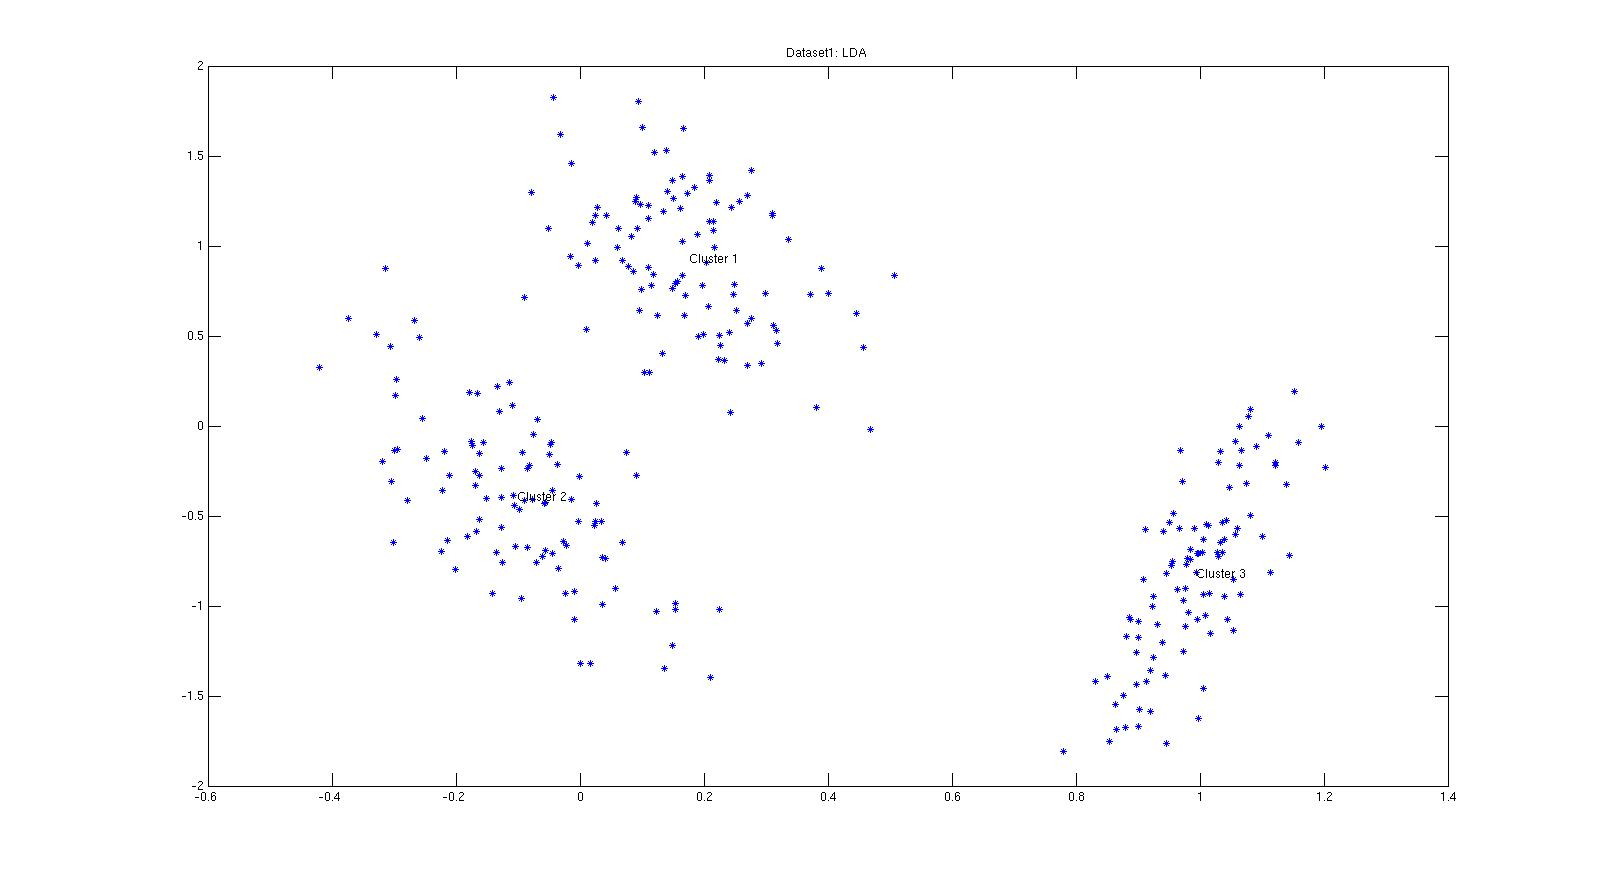
\includegraphics[scale=.2]{images/dataset1lda.jpg}

PCA:\\
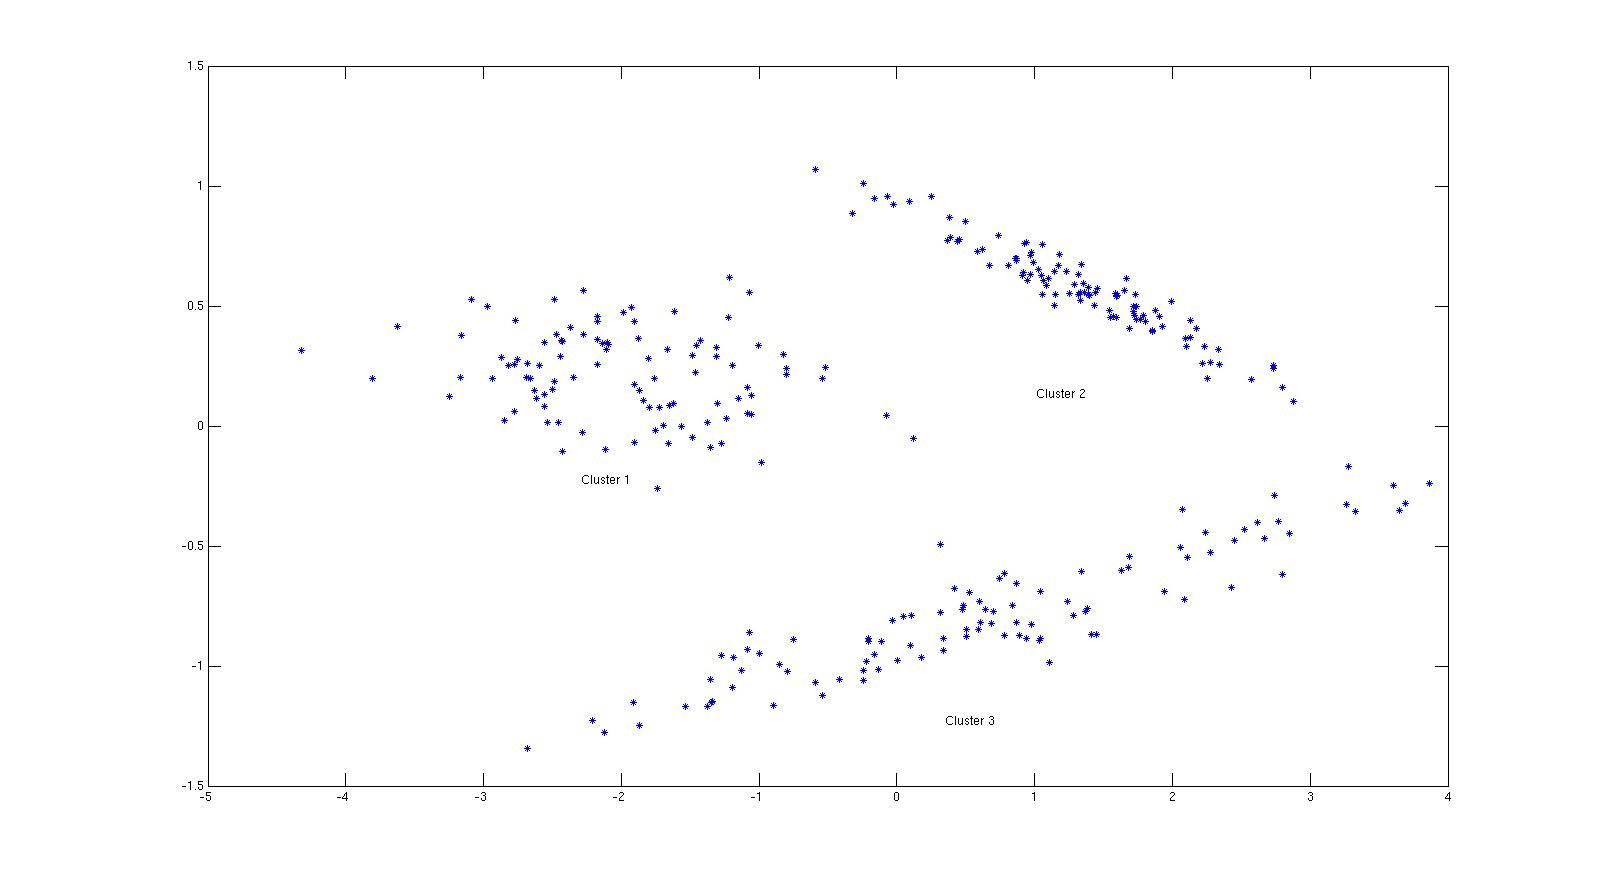
\includegraphics[scale=.2]{images/dataset1pca.jpg}


\subsection{c  (Dataset 2)}
LDA:\\
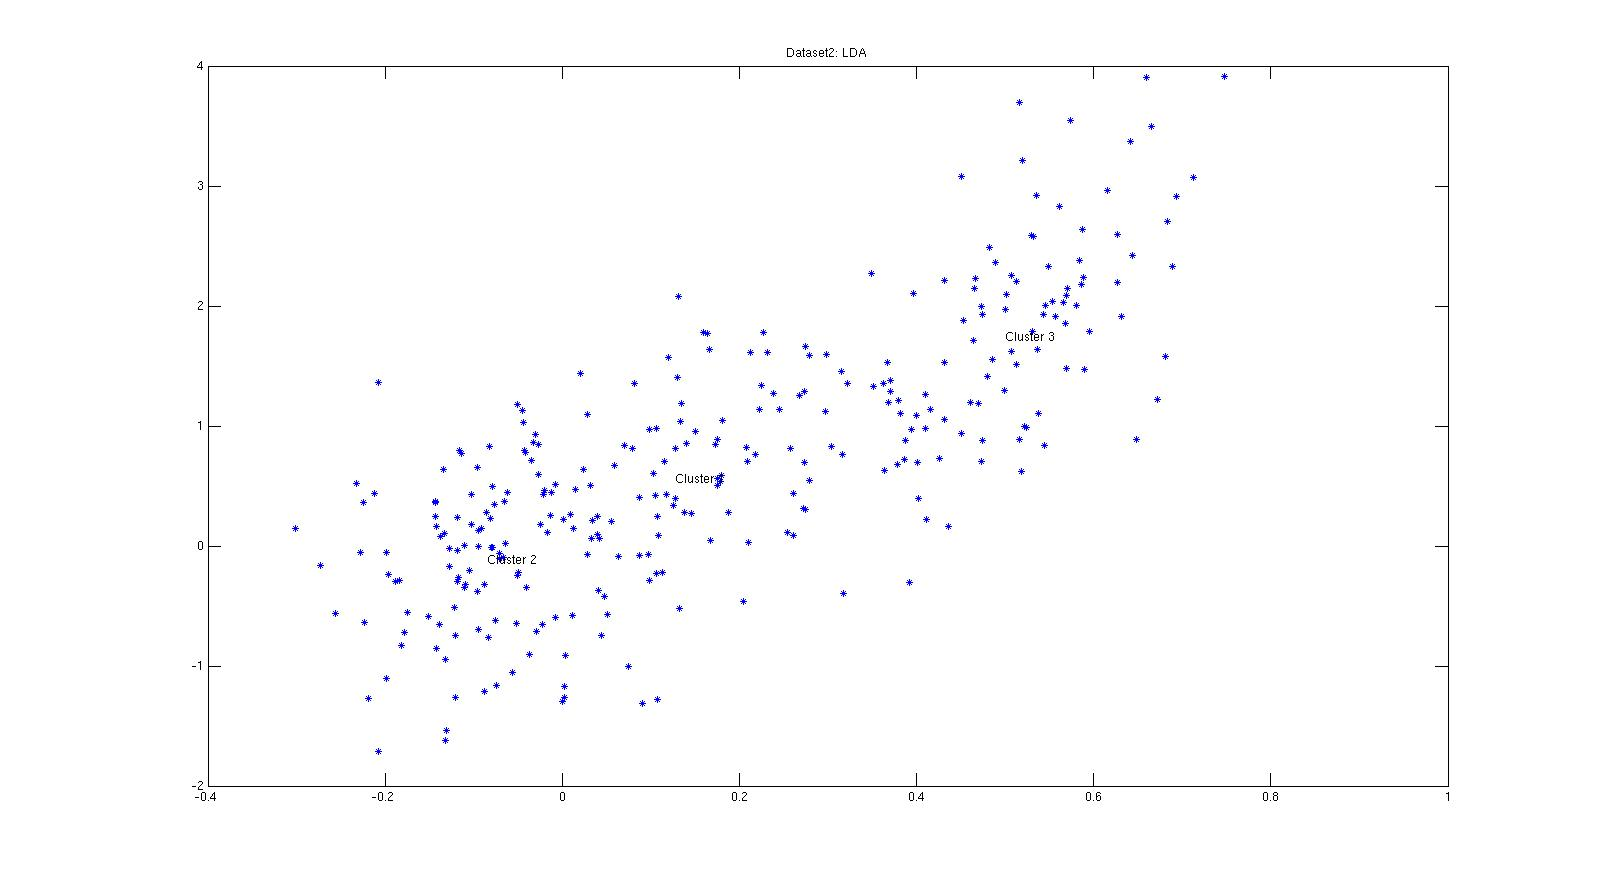
\includegraphics[scale=.2]{images/dataset2lda.jpg}

PCA:\\
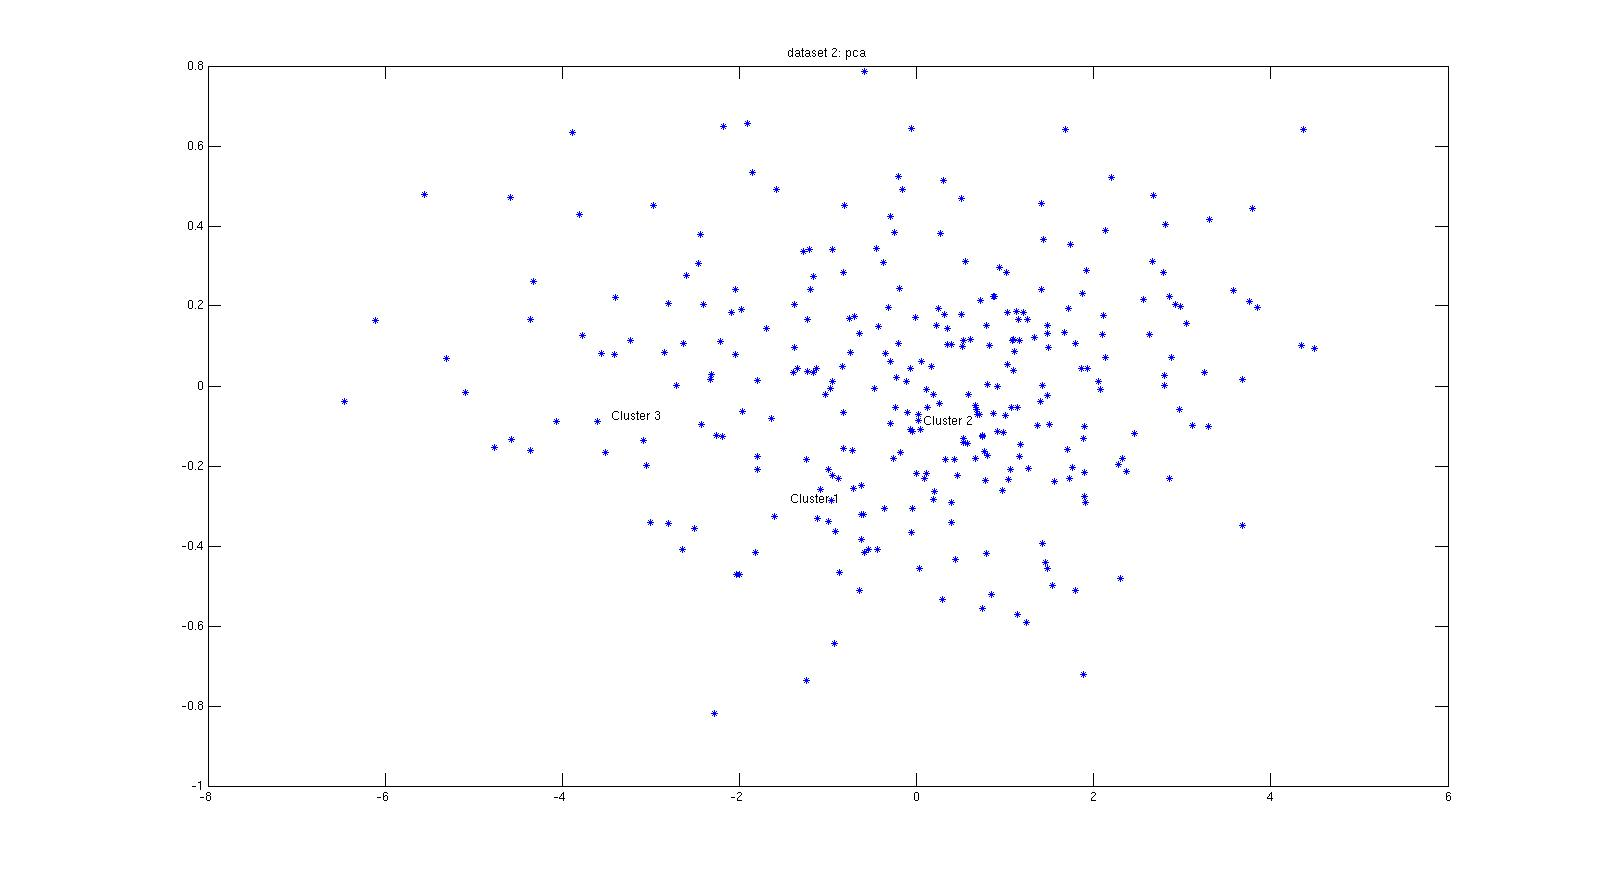
\includegraphics[scale=.2]{images/dataset2pca.jpg}


\section{3}
\subsection{Some observations}
$(m_{2} - m_{1})^{T}\covmatrix^{-1}x + c = 0$. As $\covmatrix$ is the covariance matrix, it is real and symmetric, so is $\covmatrix^{-1}$ if it exists. So, $w = \covmatrix^{-1}(m_{2} - m_{1})$. Take its SVD: $\covmatrix = US U^{T}$.

\subsection{a}
Suppose that $\covmatrix$ is non-singular. Then, the matrix of singular values $S > 0$, $S^{-1}>0$ exists. Then:
\begin{eqnarray}
w^{T}(m_{2} - m_{1}) &=& (m_{2} - m_{1})^{T}\covmatrix^{-1}(m_{2} - m_{1})\\
 &=& (m_{2} - m_{1})^{T}US^{-1} U^{T}(m_{2} - m_{1}) \\
 &=& q^{T}S^{-1}q \texttt{ (Where: $q = U^{T}(m_{2} - m_{1}) \neq 0$)} \\
 &\neq& 0\\
\end{eqnarray}

\subsection{b}
\subsubsection{Rationale}
Using the same notation as earlier: $w^{T}(m_{2} - m_{1}) = q^{T}S^{-1}q \approx 0$ for $q = U^{T}(m_{2} - m_{1}) \neq 0$ when $(m_{2} - m_{1}) \approx u_{1}$, the first singular vector and when the first singular value $s_{1}$ is very large, causing $s_{1}^{-1} \approx 0$.

The singular vectors of $\covmatrix$ happen to correspond to the major axes of the hyper-ellipses which form the level sets of the normal distribution parametrized by $\covmatrix$. As we want $s_{1}>>0$, and as this corresponds to the length of the major axes of these level sets, the spread of the data should be large. As we want $(m_{2} - m_{1}) \approx u_{1}$, the distribution should be tilted towards $m_{2} - m_{1}$. This is shown by the figure below.

\subsubsection{The figure}
The two ellipses represent level sets of 2 normal distributions: $N(x|m_{1}, \covmatrix)= N(x|m_{2}, \covmatrix) = c$ for a constant c. The arrow represents $m_{1} - m_{2}$.

For clarity, the figure does not show the dots which are the points to be clustered, but they can be imagined to be distributed according to the aforementioned distributions. The separating hyperplane, a line in this 2 dimensional case, is almost parallel to $m_{1} - m_{2}$, and $w^{T}(m_{1} - m_{2}) \approx 0$.

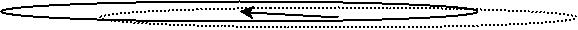
\includegraphics[scale=.5]{images/example.jpg}


% \bibliographystyle{plain}
% \bibliography{../linAlg}


\end{document}
